% Template for ICASSP-2013 paper; to be used with:
%          spconf.sty  - ICASSP/ICIP LaTeX style file, and
%          IEEEbib.bst - IEEE bibliography style file.
% --------------------------------------------------------------------------
\documentclass{article}
\usepackage{spconf,amsmath,graphicx}

% Example definitions.
% --------------------
\def\x{{\mathbf x}}
\def\L{{\cal L}}

% Title.
% ------
\title{Prostrate Cancer Detection in H\&E Stained Tissue Images}
%
% Single address.
% ---------------
\name{Ayush Jain, Chinmay Kulkarni, Aditya Rastogi}
\address{\{ajain42, ckulkarn, arastog2\}@illinois.edu}
%
% For example:
% ------------
%\address{School\\
%   Department\\
%   Address}
%
% Two addresses (uncomment and modify for two-address case).
% ----------------------------------------------------------
%\twoauthors
%  {A. Author-one, B. Author-two\sthanks{Thanks to XYZ agency for funding.}}
%   {School A-B\\
%   Department A-B\\
%   Address A-B}
%  {C. Author-three, D. Author-four\sthanks{The fourth author performed the work
%   while at ...}}
%   {School C-D\\
%   Department C-D\\
%   Address C-D}

\begin{document}
%\ninept
%
\maketitle
%
\begin{abstract}

\end{abstract}
%
\begin{keywords}
Prostrate cancer, biopsy, machine learning, image processing
\end{keywords}
%


\section{Introduction}
\label{sec:introduction}

\subsection{Background}
Prostrate cancer is the second most common cancer
among men. Several screening methodologies exist for diagnosis of prostate cancer however it is most commonly diagnosed by histopathology interpretation of Hematoxylin and Eosin (H \& E)-stained tissue sections by pathologist under a microscope. Diagnosis of prostate cancer is carried out by examining the glandular architecture of the tissue sections. The diagnosis is done in the form of the Gleason grading system \cite{gleason1966classification} under which pathologists identify the malignancy of cancer areas in tissue images on a scale of 1 to 5.Gland distributions vary with the disease grade, and the morphological features of the glands vary with the stage of cancer. However, this is prone to subjectivity and has limited intra- and inter-pathologist reproducibility, due to its heavy reliance on human interpretation. Even if only a single grade is desired, recent work has discovered that there is only a 60-70 \% agreement between pathologists on this grade.


Existing techniques to perform automated analysis of H \& E stained tissue have not had much accuracy expect in stylized toy cases. And because of the inter-disciplinary nature of the task, the problem has not attracted much attention. Most of the research has focused on distinguishing between Gleason grades (often between only two Gleason grades).In our work we focus on distinguishing cancerous tissue from non-cancerous tissue rather than distinguishing between Gleason grades for the tissue.

\subsection{Prostate Tissue Structure}
Normal Prostate tissue shown in Figure \ref{fig:tissue_structure1} is composed of gland units contained inside a fibromuscular region called stroma which holds the gland units together. Each gland unit is composed of rows of epithelial cells located around a duct, named the lumen. 

Figure \ref{fig:tissue_types} shows non-cancerous and cancerous Prostate tissue. When cancer occurs the following changes take place in the tissue depending upon the level of malignancy:
\begin{enumerate}
\item[1.] Epithelial cells replicate in an uncontrolled way, disrupting the regular arrangement of gland units.
\item[2.] The glands in the cancerous region become small, regular, and more tightly packed as
cancer progresses from benign to highly malignant. While benign,healthy tissue has large and irregular lumen regions, higher grade cancers have small, narrow lumen regions.
\end{enumerate}


\begin{figure}[!htb]
\centering
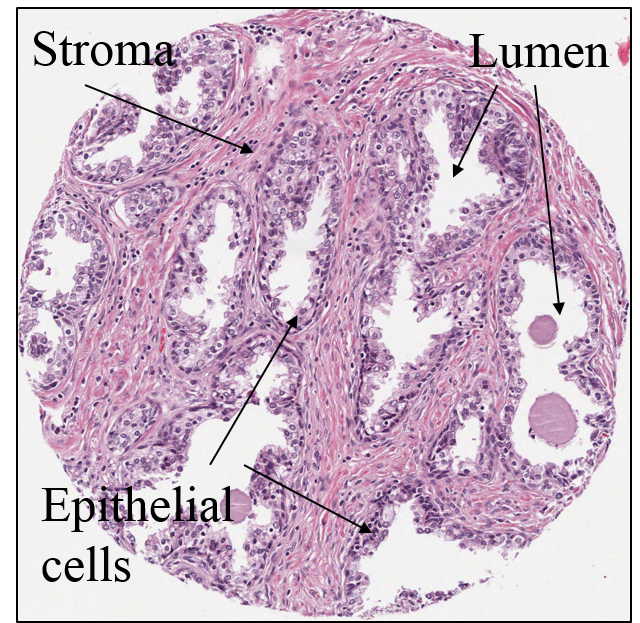
\includegraphics[scale=0.3]{figs/tissue_structure1.png}
\caption{Prostate Tissue Structure}\label{fig:tissue_structure1}
\centering
\end{figure}


\begin{figure}[!htb]
\centering
\captionsetup{justification=centering}
\begin{subfigure}{.5\textwidth}
	\centering
	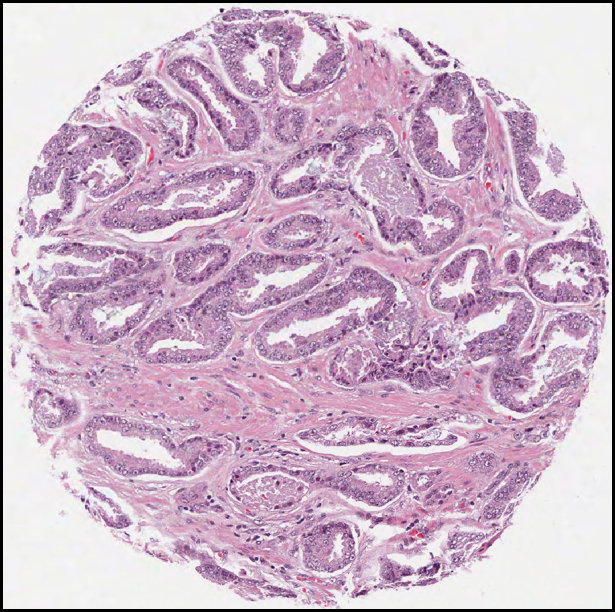
\includegraphics[scale=0.3]{figs/tissue_structure2.png}
	\caption{Benign Tissue}\label{fig:tissue_structure2}
	\centering
\end{subfigure}
\begin{subfigure}{.5\textwidth}
	\centering
	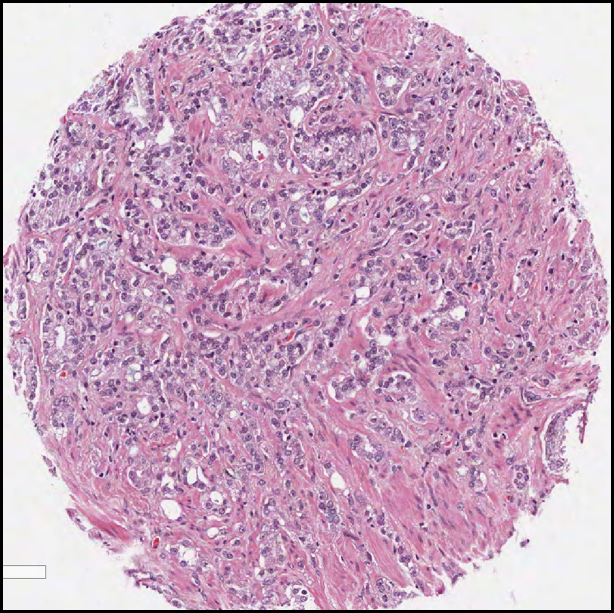
\includegraphics[scale=0.3]{figs/tissue_structure3.png}
	\caption{Malignant Tissue}\label{fig:tissue_structure2}
	\centering
\end{subfigure}
\caption{Structural changes in Prostate tissue when cancer occurs}
\label{fig:tissue_types}
\centering
\end{figure}

These changes, along with different color values identifying different regions of interest ( lumen regions are white, stroma is pink and epithelial cells are usually a dark shade of purple ) can be used to build a classification system for separating non-cancerous and cancerous images.

\section{Related Work}
There have been many different approaches tried for cancer detection in tissue stained images. \cite{automatic} segment parts of each image according to whether they are detected to be cancerous or not. In this paper, the authors make use of (Haralick features) in order to extract texture-based features. They use SVM-RFE for recursive feature selection which they apply to the entire image and evaluate their results using 10-fold cross-validation. The approach does not extract any features from the image or make use of any information about the structure of various components of the images. 
\cite{naik2007gland} make use of a more comprehensive approach. They segment parts of the image into detected gland components and subsequently extract morphological features from these components. To reduce the dimensionality of their data, they employ graph embedding and manifold learning. The features extracted for each image are very generic and do not capture much information specific to the differences in shape and size of various components of the image.
\cite{tabesh2007multifeature} make use of both morphological features as well as histogram-based features. They pre-process the images so that background colors are removed and so that the staining is made uniform. The striking fact about this paper is that they do not make use of any morphological features present in the various components of the image. In spite of using histogram-based features for their classification, the authors remove white pixels corresponding to lumen which is not intuitive. 
\cite{alexandratou2010evaluation} make use of Haralick features for extracting 13 texture characteristics using the Grey Level Co-occurence Matrix for images. They experiment with 16 different classifiers and run these classifiers over a very small data set or only about 40 images for cancer and non-cancer tissues. They obtain accuracy values of around 95\% for some of their classifiers, but the data set they use for classification is too small for this accuracy to make much sense.
The authors also count accuracy values for differentiating Gleason Score 3 and Gleason Score 4 images when they report their overall accuracy, when in fact this kind of distinction is a much easier task than differentiating cancerous images from non-cancerous images.
\cite{roula2002multispectral} make use of a novel approach wherein instead of analyzing RGB or grey scale images, they make use of the same feature vectors for a set of 16 spectral color bands. The authors apply a supervised classical Linear Discrimination method on the PCA result of the resultant combined feature vector (which is a linear combination of feature vectors for each color band) and show that the classification accuracy improves when using this spectral approach. The original feature vector contained texture-based features extracted using Haralick features. They observe better performance using the combined feature vector for 16 spectral bands over the original feature vector. The main drawback of this approach is that they are tweaking the data collection itself by observing each image as a combined feature vector of its 16 different spectral bands.

In most of the work done so far, not much effort has been put into capturing morphological features that are representative of different components of the image (lumen glands, epithelial cells and stroma). Most approaches discussed above make use of generic texture-based features without any specific processing or feature engineering for different image segments. Moreover, except for the last approach, all approaches make use of a limited number of images for testing their classifiers. In our work, we aim to focus the bulk of our effort on constructing effective and intuitive features for solving this problem. This leads to more robust features and our approach thus yields high accuracy values over data sets which are larger than those used in previous work.
\label{sec:rel_work}
\section{Patch-Based Approaches}
\label{sec:patch_based_approaches}
\section{Evaluation}
\label{sec:evaluation}
\include{conclusion}

\section{Conclusions}
\label{sec:conclusions}


% References should be produced using the bibtex program from suitable
% BiBTeX files (here: strings, refs, manuals). The IEEEbib.bst bibliography
% style file from IEEE produces unsorted bibliography list.
% -------------------------------------------------------------------------
\bibliographystyle{IEEEbib}
\bibliography{strings,refs}

\end{document}
